\documentclass[11pt, oneside]{article}   	% use "amsart" instead of "article" for AMSLaTeX format
\usepackage{geometry}                		% See geometry.pdf to learn the layout options. There are lots.
\geometry{letterpaper}                   		% ... or a4paper or a5paper or ... 
%\geometry{landscape}                		% Activate for for rotated page geometry
%\usepackage[parfill]{parskip}    		% Activate to begin paragraphs with an empty line rather than an indent
\usepackage{graphicx}				% Use pdf, png, jpg, or eps� with pdflatex; use eps in DVI mode
								% TeX will automatically convert eps --> pdf in pdflatex		
\usepackage{amssymb}
\usepackage{amsmath}

\title{Tangent to the curve $f(x)$}
%\author{The Author}
\date{}							% Activate to display a given date or no date

\graphicspath{{/Users/telliott_admin/Dropbox/Tex/png/}}

\begin{document}

\maketitle
%\section{}
% \subsection*{R code}
% \begin{lstlisting}  \end{lstlisting}
% \begin{center} 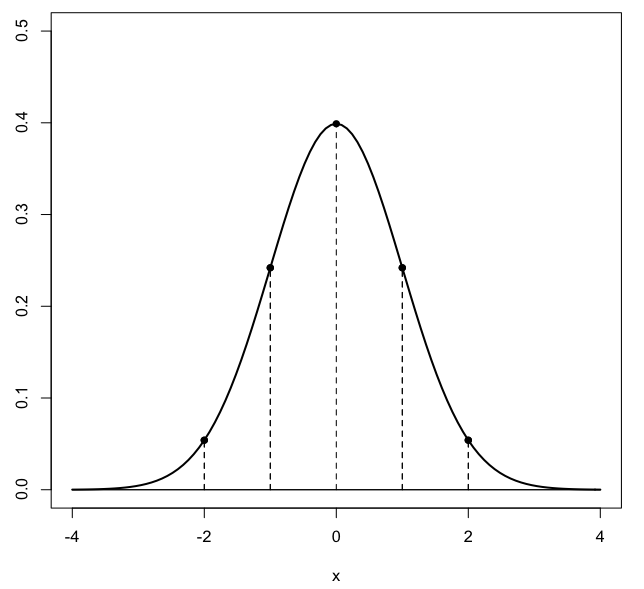
\includegraphics [scale=0.4] {gauss3.png} \end{center}
% \begin{bmatrix} a  &  b \\ c  &  d \end{bmatrix}
% \bigg |_

\large
In this short write-up we'll look at the geometric interpretation of the derivative---the beginning of an introduction to calculus.  Suppose we have a curve like in the figure, corresponding to some function.  Let's think for a minute about the general case, $f(x)$.

\begin{center} 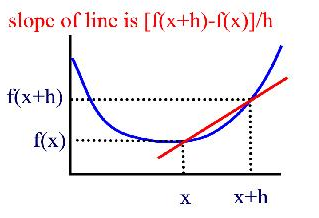
\includegraphics [scale=0.6] {tangent.png} \end{center}

We pick a point $P$ on the curve.  The value of $x$ at $P$ is $x$ (of course), and the value of $y$ is $f(x)$.  That is, the point $P$ has coordinates $P=(x,f(x))$.  Now consider moving to a point $Q$ near $P$ but also on the curve, by adding a small amount to $x$.  We could call that small amount $\Delta x$, but many books use $h$, so we'll try that.  The value of the function at $x+h$ is $f(x+h)$ and $Q=(x+h,f(x+h))$.

The slope of the line (the secant) connecting $Q$ and $P$ is
\[ \frac{\Delta y}{\Delta x} = \frac{f(x+h) - f(x)}{h} \]

This is a famous quantity, it's called the \emph{difference quotient}.
\vspace{2 mm}

\noindent The goal of this part of calculus is to find the slope of the tangent to the curve at the point $P$.  What we have is an expression for the slope of the line $PQ$, which is close but not quite the same.  To go from the secant to the tangent, we ask "what happens to this expression as $h$ gets smaller and smaller and approaches zero."  In mathematical language, we say the slope of the tangent is equal to
\begin{equation}
\boxed{\lim_{h \to 0} \ \frac{\Delta y}{\Delta x} = \frac{f(x+h) - f(x)}{h} }
\end{equation}
Let's try a couple of examples and look for a pattern.

\subsection*{Example 1.  $f(x)=x^2$}
Let's go without the limit sign to start with.  For this function, we write that the difference quotient is
\[ \frac{(x+h)^2 - x^2}{h} \]
\[ \frac{x^2 + 2xh + h^2 - x^2}{h} \]
\[ \frac{2xh + h^2}{h} \]
Now we \emph{divide by $h$}
\[ 2x + h \]
Finally, to get the slope of the tangent, we evaluate the limit part
\[ \lim_{h \to 0} \  2x + h = 2x \]

At every point on the curve $y=x^2$, the slope of the tangent line to the curve is $2x$.  So the slope at $x=0$ is $0$, and the slope at $x=2$ is $4$, and so on. We call this process of computing the difference quotient and then taking the limit as $h \to 0$, "taking the derivative."  It produces an expression which is the derivative of y with respect to x, in this case
\[ \frac{dy}{dx} = 2x \]
Another useful shorthand uses the $f$ from $f(x)$, we adopt the convention that the derivative of $f(x)$ is $f'(x)$.

If we repeat this exercise with a leading constant a (that is, for $f(x) = ax^2$), we find that every term in the numerator of the difference quotient will contain $a$, and the final result will be $2ax$.

\subsection*{Example 2.  $f(x)=\sqrt{x}, \ \ (x \ge 0)$} 
The difference quotient for this function is
\[ \frac{\sqrt{x+h} - \sqrt{x}}{h} \]
Clean up the numerator by multiplying by the conjugate
\[ \frac{\sqrt{x+h} - \sqrt{x}}{h} \ \  \frac{\sqrt{x+h} + \sqrt{x}}{\sqrt{x+h} + \sqrt{x}} \]
\[ \frac{x + h - x}{h \ (\sqrt{x})(\sqrt{x+h})}  \]
\[ \frac{h}{h \ \sqrt{x} \ \sqrt{x+h}}  \]
\[ \frac{1}{\sqrt{x} \ \sqrt{x+h}}  \]
We evaluate the limit
\[ m = \lim_{h \to 0} \  \frac{1}{\sqrt{x} \ \sqrt{x+h}} = \frac{1}{2\sqrt{x}} \]

\subsection*{Example 3.  $f(x)=1/x, \ \ (x \ne 0)$}
\Large
\[ \frac {  \frac{1}{x+h} - \frac{1}{x}  }  {h} \]
\large
Clean up the numerator
\[ \frac {  \frac{1}{x+h} - \frac{1}{x}  }  {h} \ \  \frac{(x)(x+h)}{(x)(x+h)} \]
\[ \frac {x - (x+h)}  {h\ (x) \ (x+h)} \]
\[ \frac {-h}  {h\ (x) \ (x+h)} \]
\[ -\frac {1}  {(x) \ (x+h)} \]
We put the limit part in
\[ \lim_{h \to 0} \  -\frac {1}  {(x) \ (x+h)} = - \frac{1}{x^2} \]

\subsection*{Summary}
So there's a pattern here.  We will use the notation $f'(x)$ to indicate the slope of the curve $f(x)$ at $x$, obtained as
\[ \lim_{h \to 0} \ \frac{f(x+h) - f(x)}{h} \]
\[ f(x) = x^2 \ \ \Rightarrow \ \  f'(x) = 2x \]
\[ f(x) = \sqrt{x} = x^{1/2}\ \ \Rightarrow \ \  f'(x) = \frac{1}{2}x^{-1/2}\]
\[ f(x) = \frac{1}{x} = x^{-1} \ \ \Rightarrow \ \  f'(x) = -\frac{1}{x^2} = -x^{-2} \]
The general formula is
\[ f(x) = x^n \ \ \Rightarrow \ \  f'(x) = nx^{n-1} \]
We will prove this next time.

\end{document}  